\section{壳结构、费米面与占据反馈}\label{sec:2-2}


在独立粒子壳模型中，核子在选定平均场的单粒子轨道上运动，泡利不相容原理限制了轨道的填充。这个图像给出了理解壳隙和费米面的一条起点，但当核子间的有效相互作用与占据变化同时进入计算时，壳结构也会随之改变。因而，讨论一个核为何有利于某种形变，除了寻找费米面附近的轨道，还要追问这些轨道的能量由什么占据和相互作用共同决定。

Otsuka 关于壳演化的讨论将这一问题表述为单极平均势与多体关联的反馈：跨核子数的填充可以移动壳隙，同一核内不同构型的占据重排也可以改变有效壳结构。以下采用其 2022 年独立学术论文\cite{doctoral-r1-g28-otsuka-2023-type-ii-shell-evolution}（刊于 \textit{Physics} 4, 258--285；2023 年专著章节为重印）中的单极分解，并结合 Togashi 等对 Zr 同位素的计算\cite{doctoral-r1-g28-togashi-2016-zr-mcsm-qpt}，说明这种反馈如何进入模型，以及能谱、占据和电磁强度各自能约束什么。这里的有效单粒子能量（ESPE）与形状分类均须带着指定空间、相互作用和参考态理解。



\subsection{平均场单粒子态、费米面与壳演化机制}\label{sec:2-2-1}


为引入单粒子图像，可在多体 Hamiltonian 中加减一个选定的一体平均势 $\hat{U}$。以球形参考为例，这给出单体项与剩余项的分拆：
\begin{equation}\label{eq:2-2-1}
\hat{H} = \hat{H}_0 + \hat{V}_{\mathrm{res}} = (\hat{T} + \hat{U}) + (\hat{V} - \hat{U}).
\end{equation}
这里加减同一算符是一种分拆；丢弃剩余项才构成独立粒子近似。在球形基底中，轨道由径向、轨道角动量与单粒子总角动量标号，$m$ 为磁投影。下文沿原作将轨道简记为 $j$，它同时指明所讨论的具体径向轨道。$\epsilon_{0;j}$ 是所选模型的基准单粒子能量（SPE），可包含核芯贡献与有效空间的输入，不能称为未重整化的真实裸能。

每个 $j$ 轨道最多容纳 $2j+1$ 个同类核子。在零温独立粒子参考中，质子和中子分别从低能向高能填充，最高已占据与最低未占据轨道之间标示费米能附近的边界。有关联或配对时，占据可分布于多个轨道，不能再用“最高非零占据轨道”定义费米面；此时需要结合占据分布，以及相应理论中约束平均粒子数的化学势 $\mu_p,\mu_n$ 讨论。配对如何平滑这一边界将在第 2.3 节展开。

价核子之间的相互作用还会改变各轨道感受到的平均作用。ESPE 用指定单极分解下的能量重心描述这一变化，其解释依赖 Hamiltonian、轨道基底与取期望值的多体态。单核子转移实验中，一个轨道的强度可碎裂到多个多体末态，因而其中一条最强峰也不能自动视为该轨道的 ESPE。\cite{doctoral-r1-g28-otsuka-2023-type-ii-shell-evolution}

对指定加粒反应通道、辨认的轨道 $j$ 和实际观测窗 $W$，可定义观测碎片加权重心：
\begin{equation}\label{eq:2-2-2}
\bar E^{\mathrm{obs},+}_{j,W}
=\frac{\sum_{\mu\in W}C^2S^+_{\mu j}E^+_\mu}
{\sum_{\mu\in W}C^2S^+_{\mu j}}.
\end{equation}
这里权重来自具体反应分析。若所用能量只是残核激发能，该式也仅是该激发能坐标上的窗口重心，不能直接与去粒通道或另一核的重心相并。

完整的 Baranger 型谱重心需要同一归一化 $A$ 核参考态的加、去粒子两支强度，并采用共同能量零点：$E^+_\mu=E^{A+1}_\mu-E^A$、$E^-_\nu=E^A-E^{A-1}_\nu$。在完整终态和规范产生、湮灭算符下，两支逐磁子态强度之和的分母由反对易关系给出 $g_j=2j+1$；采用约化谱学因子时还须相应换算简并度。有限窗碎片平均缺少这些完备性条件，也受反应模型与未观测强度影响，不能称为唯一、无模型的实验单粒子能量。完整谱函数关系可在附录中展开；这里仅保留它与单极能差的区别。Otsuka 的附录 A 也明确指出二者有同轨修正。\cite{doctoral-r1-g28-otsuka-2023-type-ii-shell-evolution}



\subsection{单极相互作用分解与 Type-I / Type-II 壳演化}\label{sec:2-2-2}


在选定球形价空间和两体有效相互作用后，可定义其单极部分，再以余项定义多极部分：\cite{doctoral-r1-g28-otsuka-2023-type-ii-shell-evolution}
\begin{equation}\label{eq:2-2-3}
\hat{V} = \hat{V}^{\mathrm{mono}} + \hat{V}^{\mathrm{multi}}.
\end{equation}
其中，先在正交单粒子基上定义规范化反对称态 $|\alpha\beta\rangle_A=a^\dagger_\alpha a^\dagger_\beta|0\rangle$，$\alpha=(j,m,\tau)$ 且 $\alpha\ne\beta$。同种核子的单极矩阵元写为：
\begin{equation}\label{eq:2-2-4}
V^{\mathrm{mono}}_{\tau\tau}(j,j')
=\frac{\sum_{(m,m')\ \mathrm{allowed}}
{}_A\langle jm,j'm'|\hat V|jm,j'm'\rangle_A}{D_{jj'}}.
\end{equation}
求和取 Pauli 允许的磁子态有序对；异轨 $D_{jj'}=g_jg_{j'}$，同轨 $D_{jj}=g_j(g_j-1)$。同轨交换两核子的标号会在分子和分母中同时双计，故不改变平均；改用无序对也可得到同一结果。矩阵元具有能量量纲，其交换项已由反对称态计入，不能用未反对称的裸直积替代。

在由价核子数目算符 $\hat{n}_j$ 构成的二次项表达中，同种核子（中子-中子或质子-质子）的单极相互作用哈密顿量表为：
\begin{equation}\label{eq:2-2-5}
\hat{V}^{\mathrm{mono}}_{nn} = \sum_j V^{\mathrm{mono}}_{nn}(j, j) \, \frac{1}{2} \hat{n}^n_j (\hat{n}^n_j - 1) + \sum_{j < j'} V^{\mathrm{mono}}_{nn}(j, j') \, \hat{n}^n_j \hat{n}^n_{j'}.
\end{equation}
第一项计数同轨道内不同核子构成的不重复对，并非让核子与自身作用；第二项对不同轨道只计一次。质子与中子的单极项则采用包含同位旋权重的系数：
\begin{equation}\label{eq:2-2-6}
\hat{V}^{\mathrm{mono}}_{pn} = \sum_{j, j'} \tilde{V}^{\mathrm{mono}}_{pn}(j, j') \, \hat{n}^p_j \hat{n}^n_{j'}.
\end{equation}
沿 Otsuka 式（7）—（8）的球平均与同位旋通道约定，异轨系数为
\begin{equation}\label{eq:2-2-7}
\tilde V^{\mathrm{mono}}_{pn}(j,j')
=\frac{V^{\mathrm{mono}}_0(j,j')+V^{\mathrm{mono}}_1(j,j')}{2},
\qquad j\ne j',
\end{equation}
同轨则为
\begin{equation}\label{eq:2-2-8}
\tilde V^{\mathrm{mono}}_{pn}(j,j)
=\frac12\left[
\frac{2j+2}{2j+1}V^{\mathrm{mono}}_0(j,j)
+\frac{2j}{2j+1}V^{\mathrm{mono}}_1(j,j)\right].
\end{equation}
下标 $0,1$ 指各自归一的同位旋通道重心。同轨不能继续取简单半和；这套权重也不能不加说明地套到任意电荷依赖或不同归一的 $pn$ 作用中。

取 $\hat{H}^{\mathrm{mono}}=\hat{H}_0+\hat{V}^{\mathrm{mono}}$。本文沿 Otsuka 的添粒有限差约定，中子轨道的 ESPE 算符写为：
\begin{equation}\label{eq:2-2-9}
\hat{\epsilon}^n_j = \epsilon^n_{0; j} + \sum_{j'} V^{\mathrm{mono}}_{nn}(j, j') \, \hat{n}^n_{j'} + \sum_{j'} \tilde{V}^{\mathrm{mono}}_{pn}(j', j) \, \hat{n}^p_{j'}.
\end{equation}
它对应于把轨道占据从 $n_j$ 增到 $n_j+1$ 的单极能差，实际添粒还须有空位。为看清同轨自项并确立严格的量纲与代数对照，在固定其余轨道占据的单轨简化模型中，引入具有能量量纲（MeV）的相互作用参数：令 $w_j \equiv V^{\mathrm{mono}}_{nn}(j,j)$ 代表同轨两体单极强度，标量 $U_j$ 代表其余同类轨道及质中相互作用的平均能量贡献（此处采用 $w_j, U_j$ 记号以严格区分下一节 BCS 理论中无量纲的准粒子占据振幅 $u, v$）。单轨体系能量可表为：
\begin{equation}\label{eq:2-2-10}
E_j(n) = \epsilon^n_{0;j} n + \frac{1}{2} w_j n(n-1) + U_j n.
\end{equation}
由此可严格区分添粒能 $e_j^+$、正向定义的移粒能 $e_j^-$ 以及对粒子数连续延拓的多项式导数：
\begin{equation}\label{eq:2-2-11}
\begin{aligned}
e_j^+ &= \epsilon^n_{0;j} + w_j n + U_j,\\
e_j^- &= \epsilon^n_{0;j} + w_j(n-1) + U_j,\\
\frac{\partial E_j}{\partial n} &= \epsilon^n_{0;j} + w_j\left(n - \frac{1}{2}\right) + U_j.
\end{aligned}
\end{equation}
添粒要求该轨道存在空位，移粒要求该轨道已占据核子，而连续导数并非离散整数多体体系中直接可测的单能级物理量。在简并度为 $g_j = 2j+1$ 的球对称壳层上，若归一的加粒与去粒谱强度总和分别为 $g_j - n$ 与 $n$，则两支联合的加权谱重心为：
\begin{equation}\label{eq:2-2-12}
e_j^{\mathrm{cent}} = \frac{(g_j - n) e_j^+ + n e_j^-}{g_j} = \epsilon^n_{0;j} + w_j n \left(1 - \frac{1}{g_j}\right) + U_j = e_j^+ - \frac{w_j n}{g_j}.
\end{equation}
必须强调，完整谱重心 $e_j^{\mathrm{cent}} = \epsilon^n_{0;j} + w_j n (1 - 1/g_j) + U_j$ 严格不等同于连续能量导数 $\partial E_j/\partial n = \epsilon^n_{0;j} + w_j(n - 1/2) + U_j$；两者仅在半满壳 $n = g_j/2$ 时数值重合，在偏离半满时存在本质差异 $w_j (1/2 - n/g_j)$。这是基于离散单轨两体玩具模型的严格代数推导，数值形式对应于 Otsuka 附录 A 所指示的同轨有限体系修正。

在同一固定 Hamiltonian、同一添粒约定下，定义 $\Delta n_j=\langle\Psi|\hat n_j|\Psi\rangle-\langle\Psi'|\hat n_j|\Psi'\rangle$，态间变化为：
\begin{equation}\label{eq:2-2-13}
\Delta \epsilon^n_j = \sum_{j'} V^{\mathrm{mono}}_{nn}(j, j') \, \Delta n^n_{j'} + \sum_{j'} \tilde{V}^{\mathrm{mono}}_{pn}(j', j) \, \Delta n^p_{j'}.
\end{equation}

占据差无量纲，故每项仍为能量，分别描述中子与质子占据的贡献。添粒、移粒和连续导数在上述固定单轨对照中只差态无关常数，故其态间变化一致；完整谱重心的同轨差却随占据改变，变化中仍包含残余项 $-w_j\Delta n_j/g_j$，不能无条件消去。某轨道下移与某一壳隙缩小也须分别判断，后者还要比较另一轨道。

Otsuka 用 Type-I 描述跨质子数或中子数变化的壳演化，用 Type-II 描述同一核内粒子－空穴重排引起的有效壳结构变化。同核不同态可以有不同占据，但其 Hamiltonian 无须逐态改变；改变的是相同算符在不同态中的期望值。这里两类命名用于区分比较对象，并不构成对所有壳结构变化的穷尽分类，也不意味着凡形状共存均须由同一种反馈机制解释。\cite{doctoral-r1-g28-otsuka-2023-type-ii-shell-evolution}



\subsection{力成分的微观机制与占据-形变反馈}\label{sec:2-2-3}


中心、张量和两体自旋－轨道分量均可贡献单极矩阵元。径向波函数相近，可增强某些中心作用通道的吸引，但吸排符号与强度仍取决于所选力和通道。对张量部分，常用 $j_>=l+1/2$ 与 $j_<=l-1/2$ 区分自旋－轨道伙伴。Otsuka 所讨论的张量分量显示，异侧组合可有吸引、同侧组合可有排斥；这种趋势须连同同位旋通道与径向矩阵元使用，不能称为仅由几何决定的严格选择定则，更不能据此判断总有效作用的符号。\cite{doctoral-r1-g28-otsuka-2023-type-ii-shell-evolution}

Togashi 等的 Zr 计算给出一个具体的同核比较。按 Togashi 等预印本图 3（arXiv:\allowbreak{}1606.\allowbreak{}09056v2 第 3 页）及其相邻正文说明（第 4 页），$^{98}\mathrm{Zr}$ 的 $0_1^+$ 与 $0_2^+$ 态分别具有近球形与长椭形变的模型特征，质子 $\pi0g_{9/2}$ 占据从 $0.4$ 变为 $3.5$。相应地，作者所比较的中子 $2s_{1/2}$ 至 $0g_{7/2}$ 轨道组，ESPE 展布由约 $4\ \mathrm{MeV}$ 收缩到 $2\ \mathrm{MeV}$ 以内。这些是给定 Hamil\-to\-nian 的占据期望值与模型重心，不表示实验直接测得了单粒子峰位移动。\cite{doctoral-r1-g28-togashi-2016-zr-mcsm-qpt}

在这一计算中，$\pi0g_{9/2}$ 与 $\nu0g_{7/2}$ 的中心和张量贡献相干，作者报告后者出现约 $2\ \mathrm{MeV}$ 的下移；对于 $\pi0g_{9/2}$ 与 $\nu0h_{11/2}$，两种贡献相消，净效应仍为较弱的下拉。这里约 $2\ \mathrm{MeV}$ 的轨道移动，与前述一组 ESPE 的展布变化，是相关而不同的量。单极反馈的作用是改变构型的能量代价，四极多极关联则在允许通道中建立相干，二者在此模型中共同影响形变态的能量。

允许通道尤其需要遵守宇称条件。第 2.1 节的张量选择定则表明，一体 $E2$ 算符为偶宇称，不能直接连接异宇称单粒子轨道。因此，$\nu0g_{7/2}$ 和 $\nu0h_{11/2}$ 的能量同时靠近费米能，并不赋予二者直接的 $E2$ 混合。不同宇称轨道的占据仍可通过保持多体总宇称的构型重排改变，例如允许的成对跨轨道激发；其振幅由相应两体矩阵元决定。占据重排、单极能差与同宇称允许通道中的四极相干，应分别计算后再讨论反馈，不能用“近费米轨道增多”替代这些条件。



\subsection{模型因果干预、计算方法边界与相变语义}\label{sec:2-2-4}


占据与形变在自洽解中同时变化，相关性本身还不足以划定各项相互作用的作用。Otsuka 2022 年文章所评述的 $^{154}\mathrm{Sm}$“单极冻结”计算，为此提供了受控比较。先将选定参考态 $|\Phi_{\mathrm{ref}}\rangle$ 下的单粒子期望值 $\langle\Phi_{\mathrm{ref}}|\hat\epsilon_j^\tau|\Phi_{\mathrm{ref}}\rangle$ 冻结为新的单体基准能量（新 SPE），同时从模型相互作用中移除活动的两体单极项，并完整保留全部两体多极相互作用 $\hat V^{\mathrm{multi}}$；按这一受控操作可写为：
\begin{equation}\label{eq:2-2-14}
\hat H_{\mathrm{frozen}}[\Phi_{\mathrm{ref}}]
=\sum_{\tau j}\langle\Phi_{\mathrm{ref}}|\hat\epsilon_j^\tau
|\Phi_{\mathrm{ref}}\rangle\,\hat n_j^\tau
+\hat V^{\mathrm{multi}}+C.
\end{equation}
其中 $C$ 为对齐参考能量零点所需的态无关常数，不改变激发谱。该操作的关键在于：参考态的单极效应被完全吸收入固定的一体能阶中，所切断的是后续组分变化对单极均场的动态活动反馈，绝非把两体相互作用算符粗糙地替换为一个标量常数。\cite{doctoral-r1-g28-otsuka-2023-type-ii-shell-evolution}

作者图 13 显示，以基态为参考时，建立在 $0_2^+$ 上的激发带上移约 $0.5\ \mathrm{MeV}$；以球形 Hartree–Fock 态为参考时，基态的模型形状从长椭变为三轴。后一个结果表明，在这组相互作用和参考输入下，活动单极反馈被切断后仍可出现形变。它限制了“没有活动单极重排就不能形变”的普遍断言，却不能把所有核中的驱动力一律排序为多极主导；参考态改变所得 SPE，本身就改变了比较的输入。这里引用的是综述中的模型干预结果，并非一项独立的新测量。

这类解释还须结合求解方法的边界。Togashi 等采用的蒙特卡罗壳模型（\allowbreak{}MCSM），以 Slater 行列式构造基矢，结合量子蒙特卡罗选基和变分优化，并将其投影到指定角动量与宇称后叠加。角动量投影涉及连续旋转，空间宇称则是离散对称，不能统称为连续群投影。选基依据可计算的能量等变分信息，不预先知道真实态并选择与其重叠最大的基矢。所选子空间中的求解也不等于完整价空间的精确对角化，计算精度仍须考察基组扩展和相应收敛信息。\cite{doctoral-r1-g28-togashi-2016-zr-mcsm-qpt}

原文“固定 Hamiltonian”的含义，是确定相互作用后沿 Zr 链计算时不再逐核重调。JUN45 和 SNBG3 是已有的、含经验信息的有效相互作用，$V_{\mathrm{MU}}$ 用于其余部分；该研究另对指定 $T=1$ 通道作局部调整，并使用 $^{90-96}\mathrm{Zr}$ 的 $2_1^+,4_1^+$ 与 $^{94-100}\mathrm{Zr}$ 的 $0_2^+$ 能级微调相关矩阵元。这不等于三套相互作用整体均由这批数据重新拟合。作者还报告，未作这些调整时快速转变仍出现，调整改善了谱学描述；因此既须交代经验输入，也不能将机制简单归为拟合制造。参与构造的能级仍不能计为完全独立的预测检验。

T-plot 以基矢的内禀四极矩确定在形变平面上的二维坐标，圆圈面积与相应投影基矢同所求模型本征态的重叠模方 $|\langle\Psi_{\mathrm{proj}}|\Psi\rangle|^2$ 成比例。必须注意，由于 MCSM 搜索生成的投影 Slater 行列式基矢之间彼此非正交，这些投影重叠并不构成正交完备组的互斥分解，各圆圈面积在代数上一般绝不相加为 1，亦不等于波函数在基底展开中的展开系数模平方。它们仅作为理解微观模型本征态几何组分的可视化辅助图示，不能将其误读为实验直接测得的经典形状概率密度；具体的投影归一化常数与绘图比例因实现而异。\cite{doctoral-r1-g28-togashi-2016-zr-mcsm-qpt, doctoral-r1-g28-otsuka-2023-type-ii-shell-evolution}

Togashi 等将 Zr 链的急变解释为不同重排构型弱混合所产生的量子形状相变。这是作者在其模型中的解释，沿离散中子数观察到的能谱和 $B(E2)$ 急变本身不足以单独认证相变阶数。有限维体系在特定对称性和参数路径上仍可出现精确交叉，选取最低能分支也可产生非解析点；有限性不能用来否定所有交叉或非解析选支。另一方面，这些现象与热力学极限中的相变定义须分别讨论，跨核子数的离散比较也不是自动给定的连续控制参数实验。

跨核区复用上述机制时，需要重建价空间、径向矩阵元、占据和配对条件；同名轨道或相近费米位置不足以保证同一种集体模式。第 2.3 节将进一步讨论配对怎样改变占据和激发能标，第 2.6 节则考察给定波函数对转动与形状扰动的响应。静态壳隙和形变能量提供这些问题的输入，但不能单独确定集体惯量。

\IfFileExists{Img/occupancy-centroids.pdf}{%
\begin{figure}[htbp]
\centering
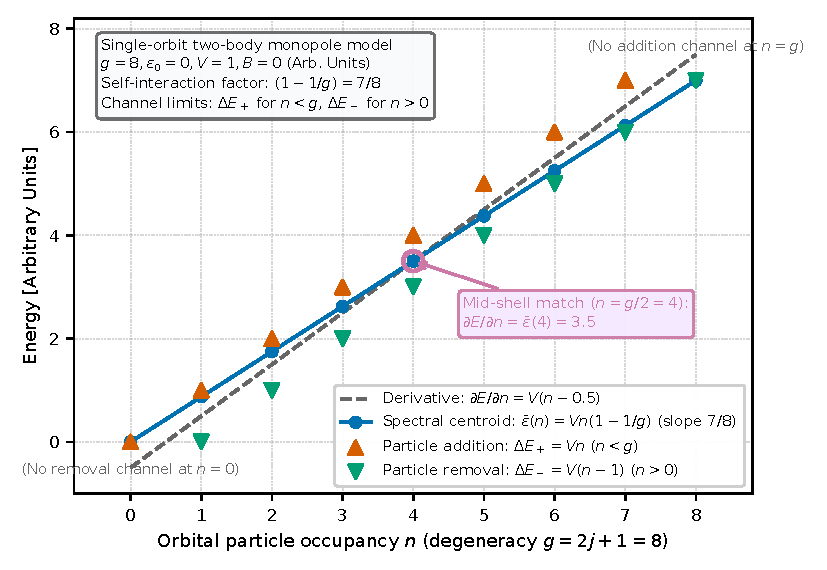
\includegraphics[width=0.85\textwidth]{Img/occupancy-centroids.pdf}
\caption{两体相互作用下的单轨道教学模型能量与重心演化对照示意图。设定轨道简并度 $g=8$，对比基准单粒子能 $e_0$、同轨两体单极相互作用强度 $w$ 与环境相互作用 $U$ 共同支配下，添粒能 $e^+$、移粒能 $e^-$、多项式连续能量导数 $\partial E/\partial n$ 以及加权谱重心 $e^{\mathrm{cent}}$ 随占据数 $n$ 的依赖关系。注意完整谱重心与连续导数在偏离半满壳层时存在本质差异（本图基于无额外多极关联的单轨两体代数模型，非真实原子核测量数据）。}
\label{fig:occupancy-centroids}
\end{figure}
}{}
